\documentclass{beamer}

\usepackage{beamerthemesplit}
\usepackage{verbatim}
\usepackage[normalem]{ulem}

\usepackage{xcolor}

\usepackage{hyperref}

\definecolor{gold}{rgb}{1.,0.84,0.}
\definecolor{brightred}{rgb}{1.,0.4,0.4}
\definecolor{mygray}{RGB}{200,200,200}
\definecolor{lightsteelblue}{RGB}{176,196,222}
\definecolor{lightskyblue}{RGB}{135,206,250}
\definecolor{cadetblue}{RGB}{95,158,160}

\usetheme{default}
\usecolortheme{mule}

\usefonttheme{serif}

\title{HSC Photometry and PSF Errors}
\author{Erin Sheldon}
\institute{Brookhaven National Laboratory}

% http://texblog.net/latex-archive/plaintex/beamer-footline-frame-number/
% to add the page (frame ) number and not screw up the bottom line
% works for split themes?
\expandafter\def\expandafter\insertshorttitle\expandafter{%
      \insertshorttitle\hfill%
        \insertframenumber\,/\,\inserttotalframenumber}

% suppress navigation bar
\beamertemplatenavigationsymbolsempty
\setbeamertemplate{footline}{}

\begin{document}

\frame{\titlepage}


\setbeamertemplate{background canvas}[vertical shading][bottom=mgray,top=mblack]

\frame
{
    \frametitle{Outline}

    \setbeamerfont*{itemize/enumerate body}{size=\Large}
    \setbeamerfont*{itemize/enumerate subbody}{parent=itemize/enumerate body}
    \setbeamerfont*{itemize/enumerate subsubbody}{parent=itemize/enumerate body}
 
    \begin{itemize}

        \item Initial HSC photometry using ngmix
        \item Comparision between coadd and multi-epoch photometry
        \item PSF Errors

    \end{itemize}

}

\frame
{
    \frametitle{Initial HSC Photometry using ngmix}

    \setbeamerfont*{itemize/enumerate body}{size=\large}
    \setbeamerfont*{itemize/enumerate subbody}{parent=itemize/enumerate body}
    \setbeamerfont*{itemize/enumerate subsubbody}{parent=itemize/enumerate body}
 
    \begin{itemize}

        \item ngmix can run on the coadd or on the original images (epochs) 

        \item multi-band multi-epoch 

        \item Can use simple masking of neighbors, the MOF deblender from DES,
            or the deblending from HSC

    \end{itemize}

}


\frame
{
    \frametitle{Initial HSC Photometry using ngmix}

    \setbeamerfont*{itemize/enumerate body}{size=\large}
    \setbeamerfont*{itemize/enumerate subbody}{parent=itemize/enumerate body}
    \setbeamerfont*{itemize/enumerate subsubbody}{parent=itemize/enumerate body}
 
    \begin{columns}
        \begin{column}{0.5\textwidth}
            \begin{itemize}

                \item The magnitudes measured using multi-epoch do not agree
                    with the coadd mags

            \end{itemize}
        \end{column}
        \begin{column}{0.5\textwidth}
            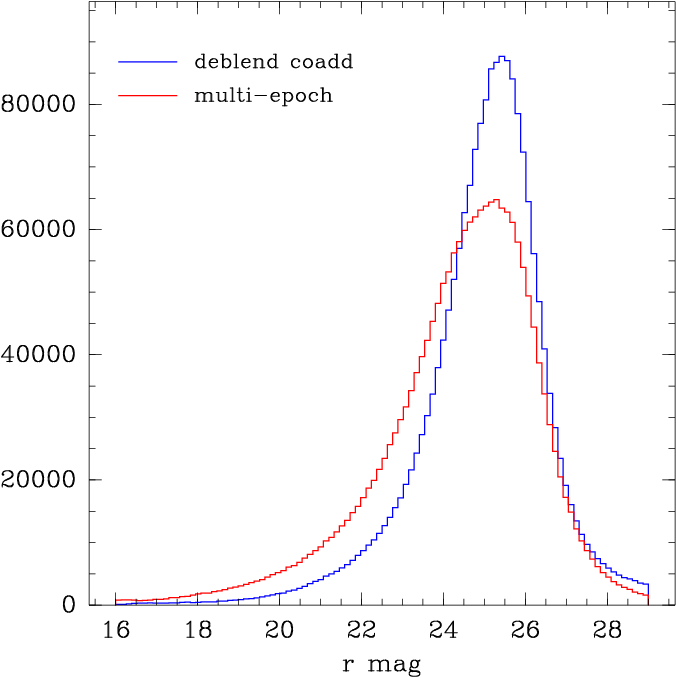
\includegraphics[width=\textwidth]{hsc-mag-compare.png}
        \end{column}
    \end{columns}
}

\frame
{
    \frametitle{Initial HSC Photometry using ngmix}

    \setbeamerfont*{itemize/enumerate body}{size=\large}
    \setbeamerfont*{itemize/enumerate subbody}{parent=itemize/enumerate body}
    \setbeamerfont*{itemize/enumerate subsubbody}{parent=itemize/enumerate body}
 
    \begin{columns}
        \begin{column}{0.5\textwidth}
            \begin{itemize}

                \item The colors are way off for multi-epoch

            \end{itemize}
        \end{column}
        \begin{column}{0.5\textwidth}
            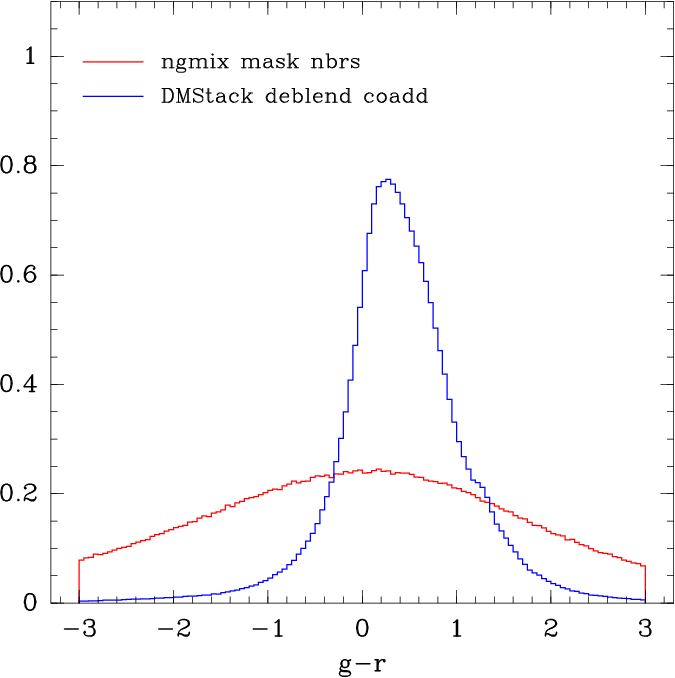
\includegraphics[width=\textwidth]{compare-me-dmstack-gmr.png}
        \end{column}
    \end{columns}
}


\frame
{
    \frametitle{Initial HSC Photometry using ngmix}

    \setbeamerfont*{itemize/enumerate body}{size=\large}
    \setbeamerfont*{itemize/enumerate subbody}{parent=itemize/enumerate body}
    \setbeamerfont*{itemize/enumerate subsubbody}{parent=itemize/enumerate body}
 
    \begin{columns}
        \begin{column}{0.5\textwidth}
            \begin{itemize}

                \item However, the ngmix coad mags agree reasonably well with
                    that from the DMStack 

            \end{itemize}
        \end{column}
        \begin{column}{0.5\textwidth}
            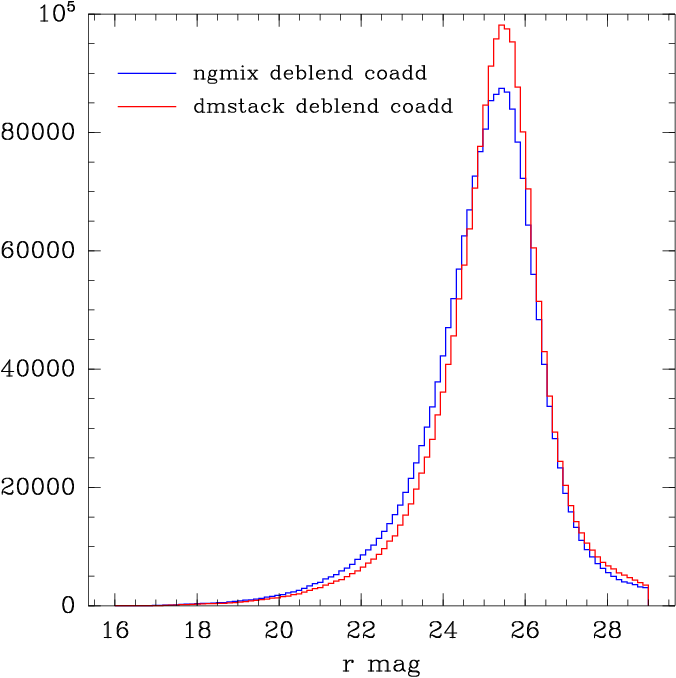
\includegraphics[width=\textwidth]{hsc-mag-compare-dmstack.png}
        \end{column}
    \end{columns}
}

\frame
{
    \frametitle{Initial HSC Photometry using ngmix}

    \setbeamerfont*{itemize/enumerate body}{size=\large}
    \setbeamerfont*{itemize/enumerate subbody}{parent=itemize/enumerate body}
    \setbeamerfont*{itemize/enumerate subsubbody}{parent=itemize/enumerate body}
 
    \begin{columns}
        \begin{column}{0.5\textwidth}
            \begin{itemize}

                \item The coadd colors are in good agreement 
                \item The difference is mostly due to noise: ngmix mags
                    are less noisy due to using information from
                    all bands

            \end{itemize}
        \end{column}
        \begin{column}{0.5\textwidth}
            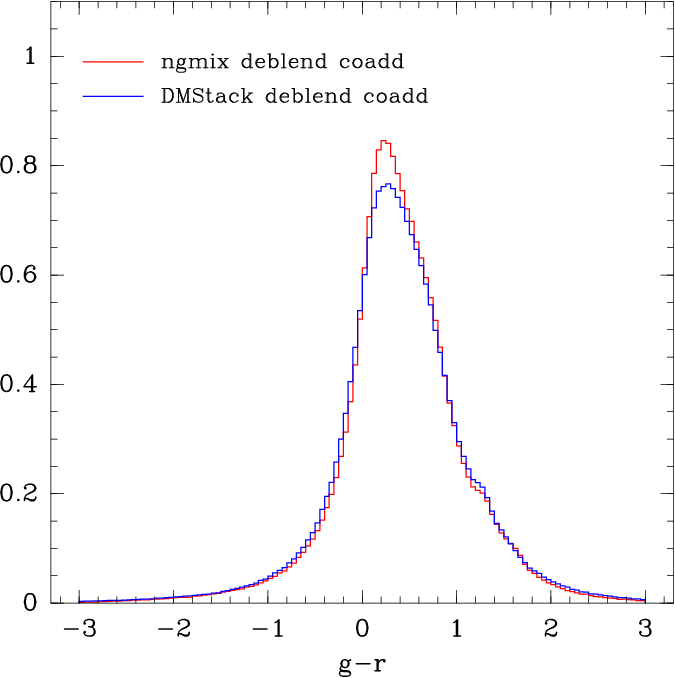
\includegraphics[width=\textwidth]{compare-dbcoadd-dmstack-gmr.png}
        \end{column}
    \end{columns}
}


\frame
{
    \frametitle{Initial HSC Photometry using ngmix}

    \setbeamerfont*{itemize/enumerate body}{size=\large}
    \setbeamerfont*{itemize/enumerate subbody}{parent=itemize/enumerate body}
    \setbeamerfont*{itemize/enumerate subsubbody}{parent=itemize/enumerate body}
 
    \begin{columns}
        \begin{column}{0.5\textwidth}
            \begin{itemize}

                \item The sizes are also different

                \item The multi-epoch sizes are systematically larger

            \end{itemize}
        \end{column}
        \begin{column}{0.5\textwidth}
            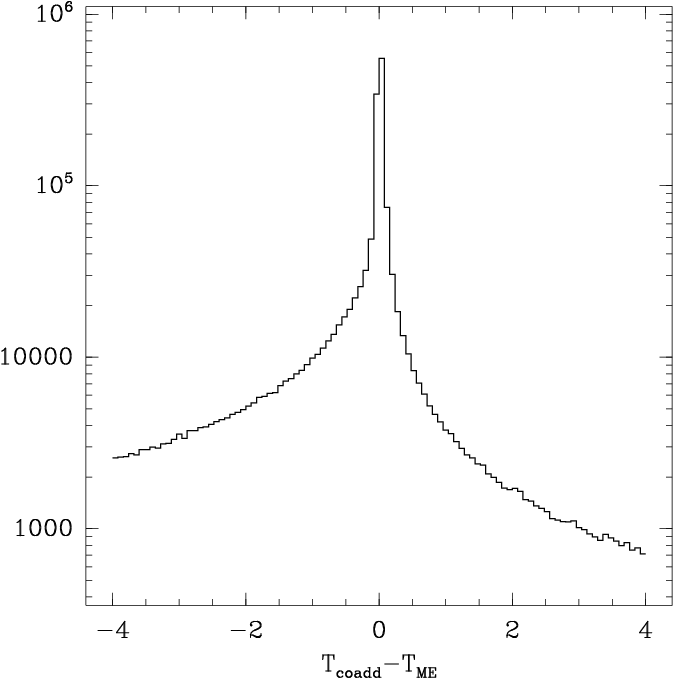
\includegraphics[width=\textwidth]{hsc-T-compare-diff.png}
        \end{column}
    \end{columns}
}


\frame
{
    \frametitle{What is going on?}

    \setbeamerfont*{itemize/enumerate body}{size=\Large}
    \setbeamerfont*{itemize/enumerate subbody}{parent=itemize/enumerate body}
    \setbeamerfont*{itemize/enumerate subsubbody}{parent=itemize/enumerate body}
 
    \begin{itemize}

        \item Something is throwing off the multi-epoch fits

        \item Reasonable agreement for coadds
            
        \item Size differences suggest a PSF effect

    \end{itemize}

}

\frame
{
    \frametitle{HSC PSF Reconstructions}

    \setbeamerfont*{itemize/enumerate body}{size=\large}
    \setbeamerfont*{itemize/enumerate subbody}{parent=itemize/enumerate body}
    \setbeamerfont*{itemize/enumerate subsubbody}{parent=itemize/enumerate body}
 
    \begin{columns}
        \begin{column}{0.5\textwidth}
            \begin{itemize}

                \item The second reconstruction I looked at

                \item There should be no negative pixels near the center

            \end{itemize}
        \end{column}
        \begin{column}{0.5\textwidth}
            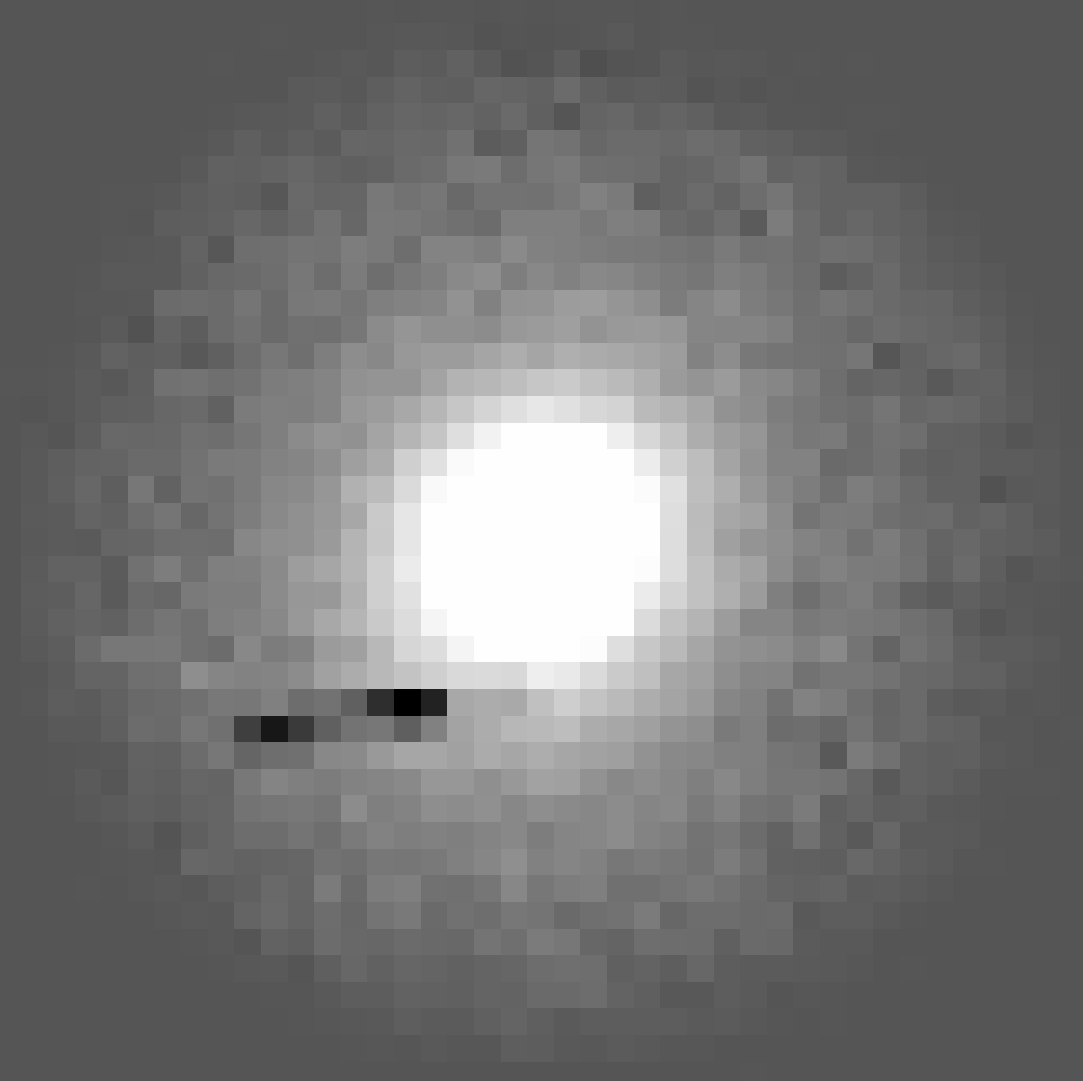
\includegraphics[width=\textwidth]{tract008766-patch66-r-object1000.png}
        \end{column}
    \end{columns}
}

\frame
{
    \frametitle{HSC PSF Reconstructions}

    \setbeamerfont*{itemize/enumerate body}{size=\large}
    \setbeamerfont*{itemize/enumerate subbody}{parent=itemize/enumerate body}
    \setbeamerfont*{itemize/enumerate subsubbody}{parent=itemize/enumerate body}
 
    \begin{center}
    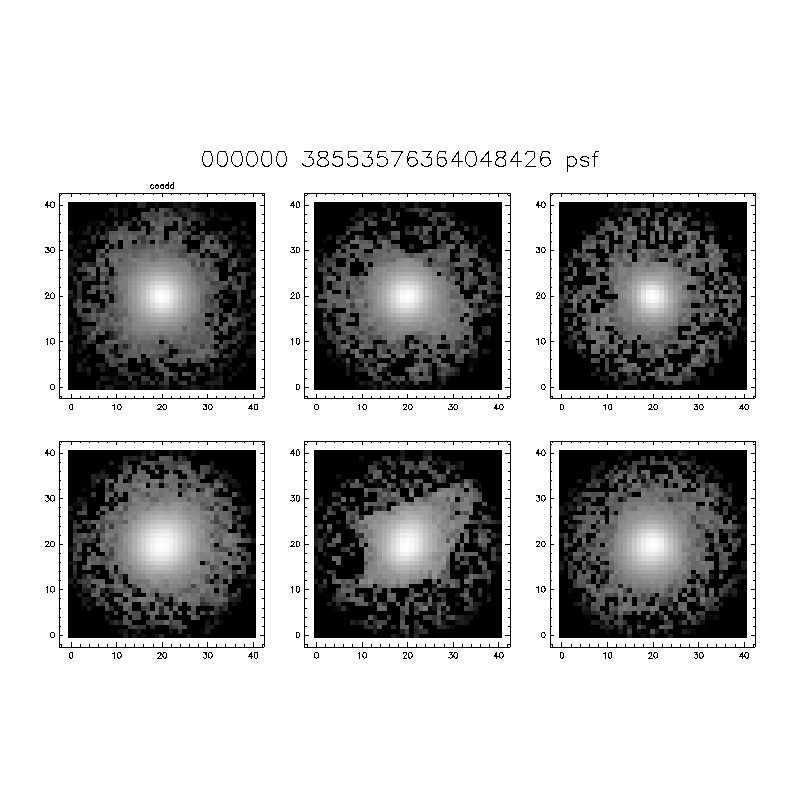
\includegraphics[height=\textheight]{tract008766-patch26_i_meds-test-medsdm-000000-psf.png}
    \end{center}
}

\frame
{
    \frametitle{HSC PSF Reconstructions}

    \setbeamerfont*{itemize/enumerate body}{size=\large}
    \setbeamerfont*{itemize/enumerate subbody}{parent=itemize/enumerate body}
    \setbeamerfont*{itemize/enumerate subsubbody}{parent=itemize/enumerate body}
 
    \begin{center}
        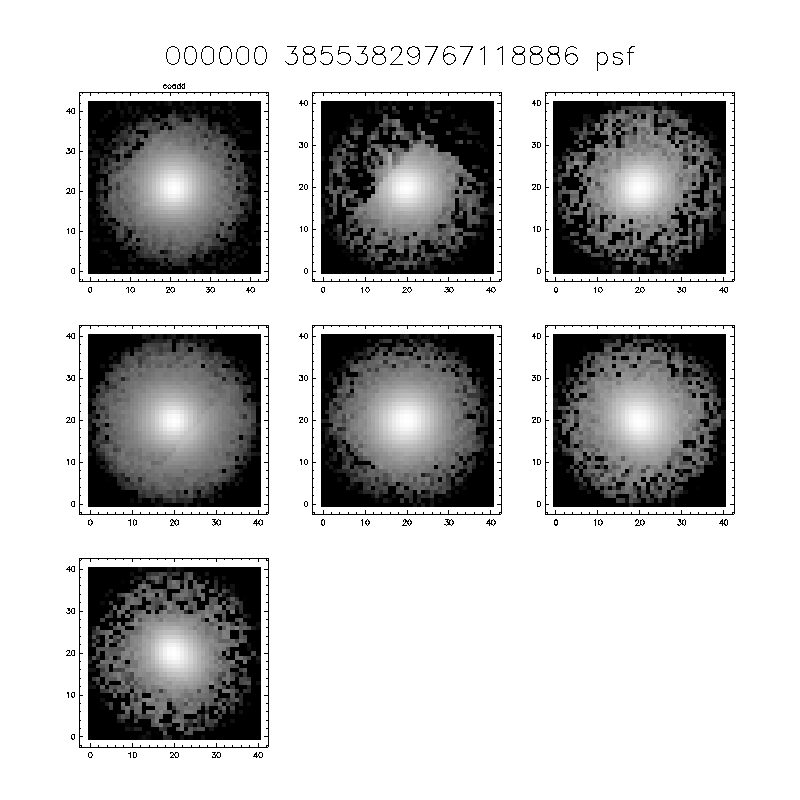
\includegraphics[height=\textheight]{tract008766-patch41_g_meds-test-medsdm-000000-psf.png}
    \end{center}
}


\frame
{
    \frametitle{HSC PSF Reconstructions}

    \setbeamerfont*{itemize/enumerate body}{size=\large}
    \setbeamerfont*{itemize/enumerate subbody}{parent=itemize/enumerate body}
    \setbeamerfont*{itemize/enumerate subsubbody}{parent=itemize/enumerate body}
 
    \begin{center}
        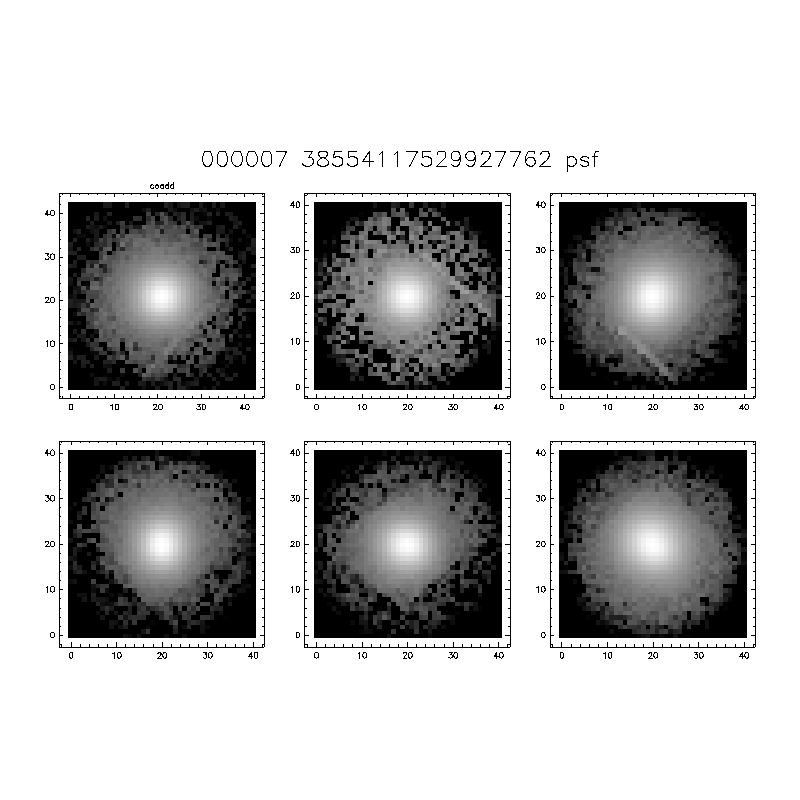
\includegraphics[height=\textheight]{tract008766-patch64_z_meds-test-medsdm-000007-psf.png}
    \end{center}
}

\frame
{
    \frametitle{Images Used for PSF Fitting (Bob Armstrong)}

    \setbeamerfont*{itemize/enumerate body}{size=\large}
    \setbeamerfont*{itemize/enumerate subbody}{parent=itemize/enumerate body}
    \setbeamerfont*{itemize/enumerate subsubbody}{parent=itemize/enumerate body}
 
    Masked images were used in the PSF fitting.  PSFEx is supposed
    to deal with these properly
    \begin{center}
        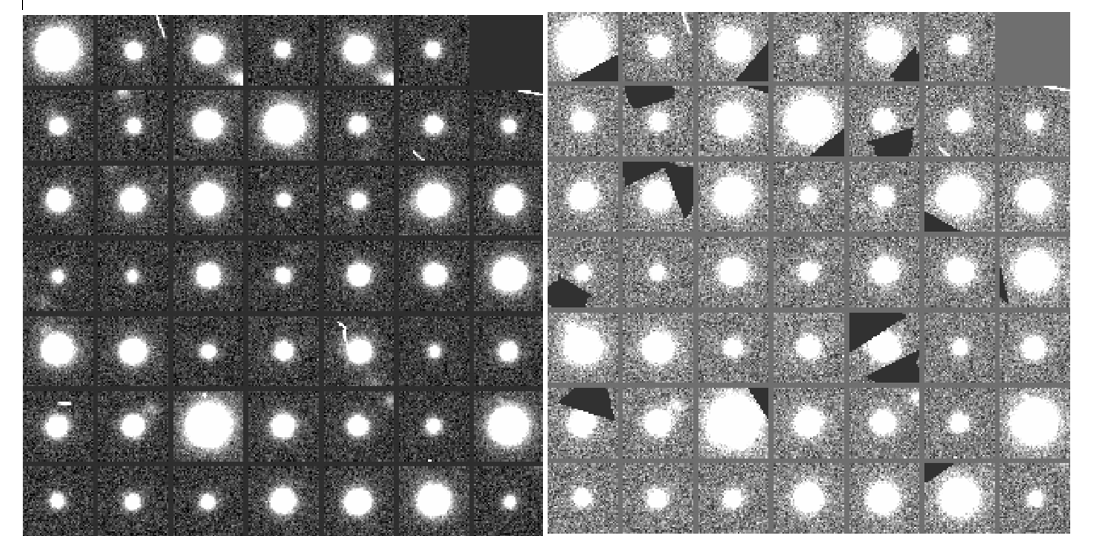
\includegraphics[width=\textwidth]{bobs-images.png}
    \end{center}
}

\frame
{
    \frametitle{Conclusions}

    \setbeamerfont*{itemize/enumerate body}{size=\Large}
    \setbeamerfont*{itemize/enumerate subbody}{parent=itemize/enumerate body}
    \setbeamerfont*{itemize/enumerate subsubbody}{parent=itemize/enumerate body}
 
    \begin{itemize}

        \item Nearly every object is affected by at least one epoch
            with a bad PSF

        \item This is causing the multi-epoch fits to be very wrong

        \item Coadds are less effected because the PSF is caodded,
            averaging down the effect.  However, the PSF is still
            wrong for the coadd

        \item My coadd fits agree with the DMStack fits because using
            the same PSF

    \end{itemize}

}





\end{document}
